\documentclass{article}

\usepackage[letterpaper]{geometry}
\usepackage{tgpagella}
\usepackage{amsmath}
\usepackage{siunitx}
\usepackage[fontsize=12pt]{fontsize}
\usepackage{tikz}
\usepackage{gnuplot-lua-tikz}
\usepackage{wrapfig}

\title{NSTGRO23 Proposal: Model-Agnostic Monte Carlo Radiation Transport}
\author{Duncan Wilkie}
\date{31 September 2022}

\begin{document}

\maketitle

\section{Project Narrative}
\label{sec:project-narrative}

Current Monte Carlo radiation transport simulation technology is showing its age.
 The user asks: ``I've got some radiation and some matter it's going to hit. Can you tell me what will happen?'' % TODO: possibly reword
Existing software, mostly agglomerations of purpose-specific FORTRAN codes that have asymptotically approached generality over the past half-century,
can answer this question reasonably well; well enough to design accelerators, reactors, and hardened silicon,
and roughly predict risks associated with living things' exposure to radiation.
The user interfaces can be recalcitrant, with many programs recently restructured or wrapped to admit friendlier interaction than an input card format,
now accessible from Python or a graphical window.
Their physical models' coverage of the radiation spectrum was often partial, their supported matter types limited,
and admissible shapes of both target and source quite specific.
These have been rectified as their market expanded, simulating ever-wider ranges of energies, elements, and geometries.

However, only the latter brought very general user control, with tetrahedral, general, and combinatorial geometry description.
As underlying models of the radiation-matter interaction grew, each code system became increasingly tied to its chosen models,
only modifiable through user-defined Fortran routines for specific edge cases where input cards were deemed insufficient.
For most purposes, this is adequate, as they are the purposes for which the models were designed.

\begin{wrapfigure}{R}{0.5\textwidth}
  \centering
  \label{fig:mcruntime}
  \scalebox{0.8}{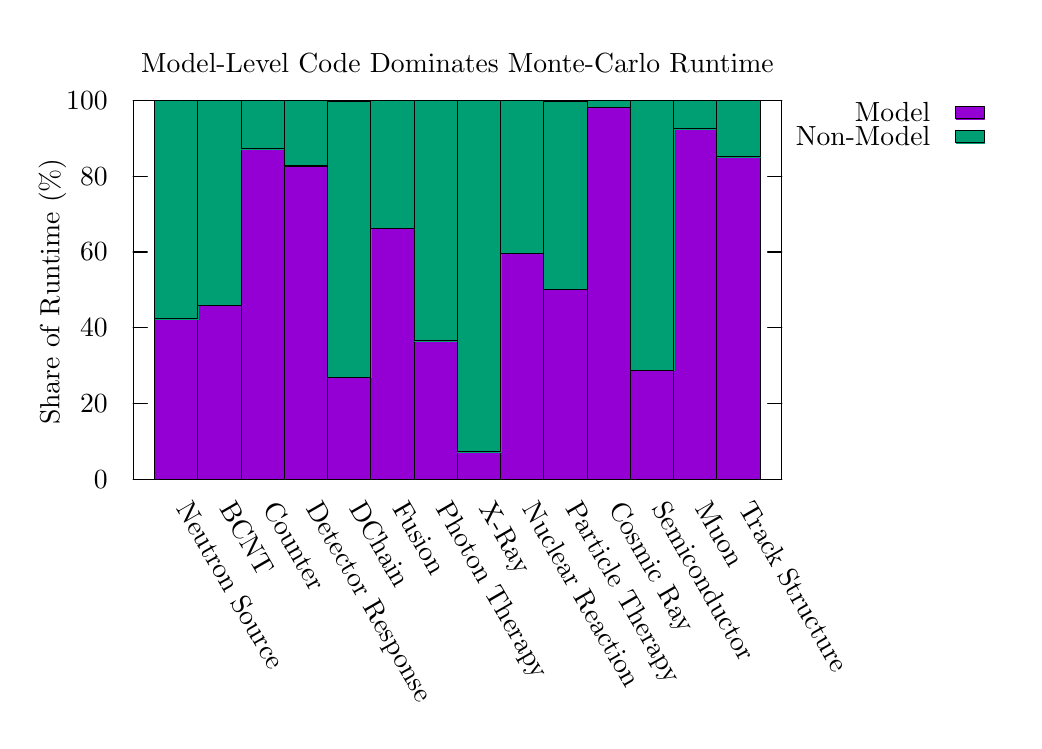
\begin{tikzpicture}[gnuplot]
%% generated with GNUPLOT 5.4p4 (Lua 5.3; terminal rev. Jun 2020, script rev. 115)
%% Fri 07 Oct 2022 04:57:14 PM CDT
\tikzset{every node/.append style={font={\fontsize{10.0pt}{12.0pt}\selectfont}}}
\path (0.000,0.000) rectangle (12.500,8.750);
\gpcolor{color=gp lt color border}
\gpsetlinetype{gp lt border}
\gpsetdashtype{gp dt solid}
\gpsetlinewidth{1.00}
\draw[gp path] (1.320,3.016)--(1.500,3.016);
\draw[gp path] (9.559,3.016)--(9.379,3.016);
\node[gp node right] at (1.136,3.016) {$0$};
\draw[gp path] (1.320,3.978)--(1.500,3.978);
\draw[gp path] (9.559,3.978)--(9.379,3.978);
\node[gp node right] at (1.136,3.978) {$20$};
\draw[gp path] (1.320,4.940)--(1.500,4.940);
\draw[gp path] (9.559,4.940)--(9.379,4.940);
\node[gp node right] at (1.136,4.940) {$40$};
\draw[gp path] (1.320,5.901)--(1.500,5.901);
\draw[gp path] (9.559,5.901)--(9.379,5.901);
\node[gp node right] at (1.136,5.901) {$60$};
\draw[gp path] (1.320,6.863)--(1.500,6.863);
\draw[gp path] (9.559,6.863)--(9.379,6.863);
\node[gp node right] at (1.136,6.863) {$80$};
\draw[gp path] (1.320,7.825)--(1.500,7.825);
\draw[gp path] (9.559,7.825)--(9.379,7.825);
\node[gp node right] at (1.136,7.825) {$100$};
\draw[gp path] (1.869,3.016)--(1.869,3.196);
\draw[gp path] (1.869,7.825)--(1.869,7.645);
\node[gp node left,rotate=-60] at (1.869,2.832) {Neutron Source};
\draw[gp path] (2.419,3.016)--(2.419,3.196);
\draw[gp path] (2.419,7.825)--(2.419,7.645);
\node[gp node left,rotate=-60] at (2.419,2.832) {BCNT};
\draw[gp path] (2.968,3.016)--(2.968,3.196);
\draw[gp path] (2.968,7.825)--(2.968,7.645);
\node[gp node left,rotate=-60] at (2.968,2.832) {Counter};
\draw[gp path] (3.517,3.016)--(3.517,3.196);
\draw[gp path] (3.517,7.825)--(3.517,7.645);
\node[gp node left,rotate=-60] at (3.517,2.832) {Detector Response};
\draw[gp path] (4.066,3.016)--(4.066,3.196);
\draw[gp path] (4.066,7.825)--(4.066,7.645);
\node[gp node left,rotate=-60] at (4.066,2.832) {DChain};
\draw[gp path] (4.616,3.016)--(4.616,3.196);
\draw[gp path] (4.616,7.825)--(4.616,7.645);
\node[gp node left,rotate=-60] at (4.616,2.832) {Fusion};
\draw[gp path] (5.165,3.016)--(5.165,3.196);
\draw[gp path] (5.165,7.825)--(5.165,7.645);
\node[gp node left,rotate=-60] at (5.165,2.832) {Photon Therapy};
\draw[gp path] (5.714,3.016)--(5.714,3.196);
\draw[gp path] (5.714,7.825)--(5.714,7.645);
\node[gp node left,rotate=-60] at (5.714,2.832) {X-Ray};
\draw[gp path] (6.263,3.016)--(6.263,3.196);
\draw[gp path] (6.263,7.825)--(6.263,7.645);
\node[gp node left,rotate=-60] at (6.263,2.832) {Nuclear Reaction};
\draw[gp path] (6.813,3.016)--(6.813,3.196);
\draw[gp path] (6.813,7.825)--(6.813,7.645);
\node[gp node left,rotate=-60] at (6.813,2.832) {Particle Therapy};
\draw[gp path] (7.362,3.016)--(7.362,3.196);
\draw[gp path] (7.362,7.825)--(7.362,7.645);
\node[gp node left,rotate=-60] at (7.362,2.832) {Cosmic Ray};
\draw[gp path] (7.911,3.016)--(7.911,3.196);
\draw[gp path] (7.911,7.825)--(7.911,7.645);
\node[gp node left,rotate=-60] at (7.911,2.832) {Semiconductor};
\draw[gp path] (8.460,3.016)--(8.460,3.196);
\draw[gp path] (8.460,7.825)--(8.460,7.645);
\node[gp node left,rotate=-60] at (8.460,2.832) {Muon};
\draw[gp path] (9.010,3.016)--(9.010,3.196);
\draw[gp path] (9.010,7.825)--(9.010,7.645);
\node[gp node left,rotate=-60] at (9.010,2.832) {Track Structure};
\draw[gp path] (1.320,7.825)--(1.320,3.016)--(9.559,3.016)--(9.559,7.825)--cycle;
\node[gp node center,rotate=-270] at (0.292,5.420) {Share of Runtime (\%)};
\node[gp node right] at (11.583,7.671) {Model};
\gpfill{rgb color={0.580,0.000,0.827}} (11.767,7.594)--(12.131,7.594)--(12.131,7.748)--(11.767,7.748)--cycle;
\draw[gp path] (11.767,7.594)--(12.131,7.594)--(12.131,7.748)--(11.767,7.748)--cycle;
\gpfill{rgb color={0.580,0.000,0.827}} (1.595,3.016)--(2.145,3.016)--(2.145,5.053)--(1.595,5.053)--cycle;
\draw[gp path] (1.595,3.016)--(1.595,5.052)--(2.144,5.052)--(2.144,3.016)--cycle;
\gpfill{rgb color={0.580,0.000,0.827}} (2.144,3.016)--(2.694,3.016)--(2.694,5.225)--(2.144,5.225)--cycle;
\draw[gp path] (2.144,3.016)--(2.144,5.224)--(2.693,5.224)--(2.693,3.016)--cycle;
\gpfill{rgb color={0.580,0.000,0.827}} (2.693,3.016)--(3.243,3.016)--(3.243,7.213)--(2.693,7.213)--cycle;
\draw[gp path] (2.693,3.016)--(2.693,7.212)--(3.242,7.212)--(3.242,3.016)--cycle;
\gpfill{rgb color={0.580,0.000,0.827}} (3.242,3.016)--(3.793,3.016)--(3.793,6.994)--(3.242,6.994)--cycle;
\draw[gp path] (3.242,3.016)--(3.242,6.993)--(3.792,6.993)--(3.792,3.016)--cycle;
\gpfill{rgb color={0.580,0.000,0.827}} (3.792,3.016)--(4.342,3.016)--(4.342,4.308)--(3.792,4.308)--cycle;
\draw[gp path] (3.792,3.016)--(3.792,4.307)--(4.341,4.307)--(4.341,3.016)--cycle;
\gpfill{rgb color={0.580,0.000,0.827}} (4.341,3.016)--(4.891,3.016)--(4.891,6.205)--(4.341,6.205)--cycle;
\draw[gp path] (4.341,3.016)--(4.341,6.204)--(4.890,6.204)--(4.890,3.016)--cycle;
\gpfill{rgb color={0.580,0.000,0.827}} (4.890,3.016)--(5.441,3.016)--(5.441,4.777)--(4.890,4.777)--cycle;
\draw[gp path] (4.890,3.016)--(4.890,4.776)--(5.440,4.776)--(5.440,3.016)--cycle;
\gpfill{rgb color={0.580,0.000,0.827}} (5.440,3.016)--(5.990,3.016)--(5.990,3.366)--(5.440,3.366)--cycle;
\draw[gp path] (5.440,3.016)--(5.440,3.365)--(5.989,3.365)--(5.989,3.016)--cycle;
\gpfill{rgb color={0.580,0.000,0.827}} (5.989,3.016)--(6.539,3.016)--(6.539,5.884)--(5.989,5.884)--cycle;
\draw[gp path] (5.989,3.016)--(5.989,5.883)--(6.538,5.883)--(6.538,3.016)--cycle;
\gpfill{rgb color={0.580,0.000,0.827}} (6.538,3.016)--(7.088,3.016)--(7.088,5.431)--(6.538,5.431)--cycle;
\draw[gp path] (6.538,3.016)--(6.538,5.430)--(7.087,5.430)--(7.087,3.016)--cycle;
\gpfill{rgb color={0.580,0.000,0.827}} (7.087,3.016)--(7.638,3.016)--(7.638,7.737)--(7.087,7.737)--cycle;
\draw[gp path] (7.087,3.016)--(7.087,7.736)--(7.637,7.736)--(7.637,3.016)--cycle;
\gpfill{rgb color={0.580,0.000,0.827}} (7.637,3.016)--(8.187,3.016)--(8.187,4.399)--(7.637,4.399)--cycle;
\draw[gp path] (7.637,3.016)--(7.637,4.398)--(8.186,4.398)--(8.186,3.016)--cycle;
\gpfill{rgb color={0.580,0.000,0.827}} (8.186,3.016)--(8.736,3.016)--(8.736,7.469)--(8.186,7.469)--cycle;
\draw[gp path] (8.186,3.016)--(8.186,7.468)--(8.735,7.468)--(8.735,3.016)--cycle;
\gpfill{rgb color={0.580,0.000,0.827}} (8.735,3.016)--(9.285,3.016)--(9.285,7.112)--(8.735,7.112)--cycle;
\draw[gp path] (8.735,3.016)--(8.735,7.111)--(9.284,7.111)--(9.284,3.016)--cycle;
\node[gp node right] at (11.583,7.363) {Non-Model};
\gpfill{rgb color={0.000,0.620,0.451}} (11.767,7.286)--(12.131,7.286)--(12.131,7.440)--(11.767,7.440)--cycle;
\draw[gp path] (11.767,7.286)--(12.131,7.286)--(12.131,7.440)--(11.767,7.440)--cycle;
\gpfill{rgb color={0.000,0.620,0.451}} (1.595,5.052)--(2.145,5.052)--(2.145,7.826)--(1.595,7.826)--cycle;
\draw[gp path] (1.595,5.052)--(1.595,7.825)--(2.144,7.825)--(2.144,5.052)--cycle;
\gpfill{rgb color={0.000,0.620,0.451}} (2.144,5.224)--(2.694,5.224)--(2.694,7.825)--(2.144,7.825)--cycle;
\draw[gp path] (2.144,5.224)--(2.144,7.824)--(2.693,7.824)--(2.693,5.224)--cycle;
\gpfill{rgb color={0.000,0.620,0.451}} (2.693,7.212)--(3.243,7.212)--(3.243,7.823)--(2.693,7.823)--cycle;
\draw[gp path] (2.693,7.212)--(2.693,7.822)--(3.242,7.822)--(3.242,7.212)--cycle;
\gpfill{rgb color={0.000,0.620,0.451}} (3.242,6.993)--(3.793,6.993)--(3.793,7.826)--(3.242,7.826)--cycle;
\draw[gp path] (3.242,6.993)--(3.242,7.825)--(3.792,7.825)--(3.792,6.993)--cycle;
\gpfill{rgb color={0.000,0.620,0.451}} (3.792,4.307)--(4.342,4.307)--(4.342,7.818)--(3.792,7.818)--cycle;
\draw[gp path] (3.792,4.307)--(3.792,7.817)--(4.341,7.817)--(4.341,4.307)--cycle;
\gpfill{rgb color={0.000,0.620,0.451}} (4.341,6.204)--(4.891,6.204)--(4.891,7.826)--(4.341,7.826)--cycle;
\draw[gp path] (4.341,6.204)--(4.341,7.825)--(4.890,7.825)--(4.890,6.204)--cycle;
\gpfill{rgb color={0.000,0.620,0.451}} (4.890,4.776)--(5.441,4.776)--(5.441,7.826)--(4.890,7.826)--cycle;
\draw[gp path] (4.890,4.776)--(4.890,7.825)--(5.440,7.825)--(5.440,4.776)--cycle;
\gpfill{rgb color={0.000,0.620,0.451}} (5.440,3.365)--(5.990,3.365)--(5.990,7.826)--(5.440,7.826)--cycle;
\draw[gp path] (5.440,3.365)--(5.440,7.825)--(5.989,7.825)--(5.989,3.365)--cycle;
\gpfill{rgb color={0.000,0.620,0.451}} (5.989,5.883)--(6.539,5.883)--(6.539,7.826)--(5.989,7.826)--cycle;
\draw[gp path] (5.989,5.883)--(5.989,7.825)--(6.538,7.825)--(6.538,5.883)--cycle;
\gpfill{rgb color={0.000,0.620,0.451}} (6.538,5.430)--(7.088,5.430)--(7.088,7.816)--(6.538,7.816)--cycle;
\draw[gp path] (6.538,5.430)--(6.538,7.815)--(7.087,7.815)--(7.087,5.430)--cycle;
\gpfill{rgb color={0.000,0.620,0.451}} (7.087,7.736)--(7.638,7.736)--(7.638,7.822)--(7.087,7.822)--cycle;
\draw[gp path] (7.087,7.736)--(7.087,7.821)--(7.637,7.821)--(7.637,7.736)--cycle;
\gpfill{rgb color={0.000,0.620,0.451}} (7.637,4.398)--(8.187,4.398)--(8.187,7.826)--(7.637,7.826)--cycle;
\draw[gp path] (7.637,4.398)--(7.637,7.825)--(8.186,7.825)--(8.186,4.398)--cycle;
\gpfill{rgb color={0.000,0.620,0.451}} (8.186,7.468)--(8.736,7.468)--(8.736,7.826)--(8.186,7.826)--cycle;
\draw[gp path] (8.186,7.468)--(8.186,7.825)--(8.735,7.825)--(8.735,7.468)--cycle;
\gpfill{rgb color={0.000,0.620,0.451}} (8.735,7.111)--(9.285,7.111)--(9.285,7.826)--(8.735,7.826)--cycle;
\draw[gp path] (8.735,7.111)--(8.735,7.825)--(9.284,7.825)--(9.284,7.111)--cycle;
\draw[gp path] (1.320,7.825)--(1.320,3.016)--(9.559,3.016)--(9.559,7.825)--cycle;
\node[gp node center] at (5.439,8.287) {Model-Level Code Dominates Monte-Carlo Runtime};
%% coordinates of the plot area
\gpdefrectangularnode{gp plot 1}{\pgfpoint{1.320cm}{3.016cm}}{\pgfpoint{9.559cm}{7.825cm}}
\end{tikzpicture}
%% gnuplot variables
}
  \caption{Self-sourced investigation; these are PHITS-provided examples that are all relatively short ($<$2min runtime).
  The slight correlation seen (the $x$-axis is ordered by total runtime) can be expected to shrink, as most non-model code is one-time.}
\end{wrapfigure}

Space medical physics, by contrast, sees such large discrepancy between prediction and observation that model-level innovation is likely to be necessary.
Current research uses Monte Carlo tools widely, to probe observed discrepancy between animal and human resilience to exposure,
for automated design of optimal spacecraft shielding, and to create phantom models for beamline measurements. % TODO: better/refined examples
At the same time, current research attempts to improve mathematical modeling of the radiation interactions, e.g. for thick targets like spacecraft shielding.
The former science would benefit from swift integration of the latter's advancements,
but as-is there are few possibilities to do so outside correspondence with the developers.

I propose the development of a model-agnostic transport program core, capable of interfacing with current model code and new model code as the user sees fit.
The user will provide programmatic description of the desired geometry and radiation sources, and a selection of models to use under different conditions.
The program will mediate between this representation and the representation expected by the underlying models, switching between them as instructed,
and returning aggregate results to the user.
It should provide a scheme for parallel and distributed computation as well, enabling the use of standard high-performance computing resources.
The user ought to be able to use the program as a module in a common, general-purpose programming language in which extensive tooling for data analysis
and further computation is available.

Setup and marshaling of user input is a minimal proportion of CPU and developer time in existing codes.
% TODO: estimate line counts
As this software





\end{document}
